\documentclass[letterpaper, reqno,11pt]{article}
\usepackage[margin=1.0in]{geometry}
\usepackage{color,latexsym,amsmath,amssymb,graphicx, float}
\usepackage{hyperref}

\hypersetup{
colorlinks=true,
linkcolor=magenta,
filecolor=magenta,
urlcolor=cyan,
}

\graphicspath{ {images/} }

\newcommand{\RR}{\mathbb{R}}
\newcommand{\CC}{\mathbb{C}}
\newcommand{\ZZ}{\mathbb{Z}}
\newcommand{\QQ}{\mathbb{Q}}
\newcommand{\NN}{\mathbb{N}}
\newcommand{\st}{\text{ s.t.}\ }

\begin{document}
\pagenumbering{arabic}
\title{PHYS 304 Assignment 1}
\date{17/01/22}
\author{Xander Naumenko}
\maketitle

{\noindent\bf Question 1a.} From the problem we know that $<j> =21$. Plugging the values into the formula, this becomes: 

\[
<j^2> =\sum_j (j-<j>)^2 N(j)=\frac{1}{14}(14^2+15^2+16^2\cdot 3+22^2\cdot 2+24^2\cdot 2+25^2\cdot 5)=459.6
.\] 

Using the fact we already know $<j> =21$ then clearly $<j>^2=441$. 

{\noindent\bf Question 1b.} Summing each of the terms: 

\[
\sigma=\sqrt{\frac{1}{14}\left( 7^2+6^2+3\cdot 5^2+2\cdot 1^2+2\cdot 3^2+5\cdot 4^2 \right)} =4.309
.\] 

{\noindent\bf Question 1c.} Using equation 1.12: 

\[
\sigma=\sqrt{\left<j^2 \right>-\left<j \right>^2} =4.309
.\] 

As expected this verifies the result of part b. 

{\noindent\bf Question 2a.} From the example we know that the probability density for the rock is 

\[
\rho=\frac{1}{2\sqrt{hx} }
.\] 

The example also found that $\left<x \right> =\frac{h}{3}$. Thus the standard deviation is 

\[
\sigma=\sqrt{\int_0^h \frac{(x-\frac{h}{3})^2}{2\sqrt{hx} }dx } =\sqrt{\frac{h^{\frac{5}{2}}}{5\sqrt{h} }-\frac{2h^{\frac{5}{2}}h}{9\sqrt{h} }+\frac{h^{\frac{5}{2}}}{9\sqrt{h} }}=\sqrt{\frac{h^2}{5}-\frac{h^2}{9}}=\frac{2h}{3\sqrt{5} }
.\] 

{\noindent\bf Question 2b.} The probability is the following integral: 

\[
1-\int_{\frac{h}{3}-\frac{2h}{3\sqrt{5} }}^{\frac{h}{3}+\frac{2h}{3\sqrt{5}}}\frac{1}{2\sqrt{hx}}=1-\sqrt{\frac{x}{h}} \bigg|_{\frac{h}{3}-\frac{2h}{3\sqrt{5} }}^{\frac{h}{3}+\frac{2h}{3\sqrt{5}}}=1-\sqrt{\frac{1}{3}+\frac{2}{3\sqrt{5} }} +\sqrt{\frac{1}{3}-\frac{2}{3\sqrt{5}}}
.\] 

{\noindent\bf Question 3a.} To normalize we first find the integral of the wavefunction squared: 

\[
\int_0^a \left(\frac{x}{a}\right)^2dx + \int_a^b \left(\frac{(b-x)}{b-a}\right)^2dx=\frac{a}{3}+\frac{(b-a)}{3}=\sqrt{\frac{b}{3}}
.\] 

Thus to normalize the wavefunction you must choose $A=\sqrt{\frac{3}{b}}$

{\noindent\bf Question 3b.} See the graph in figure \ref{fig:q3}. 

\begin{figure}[htpb]
    \centering
    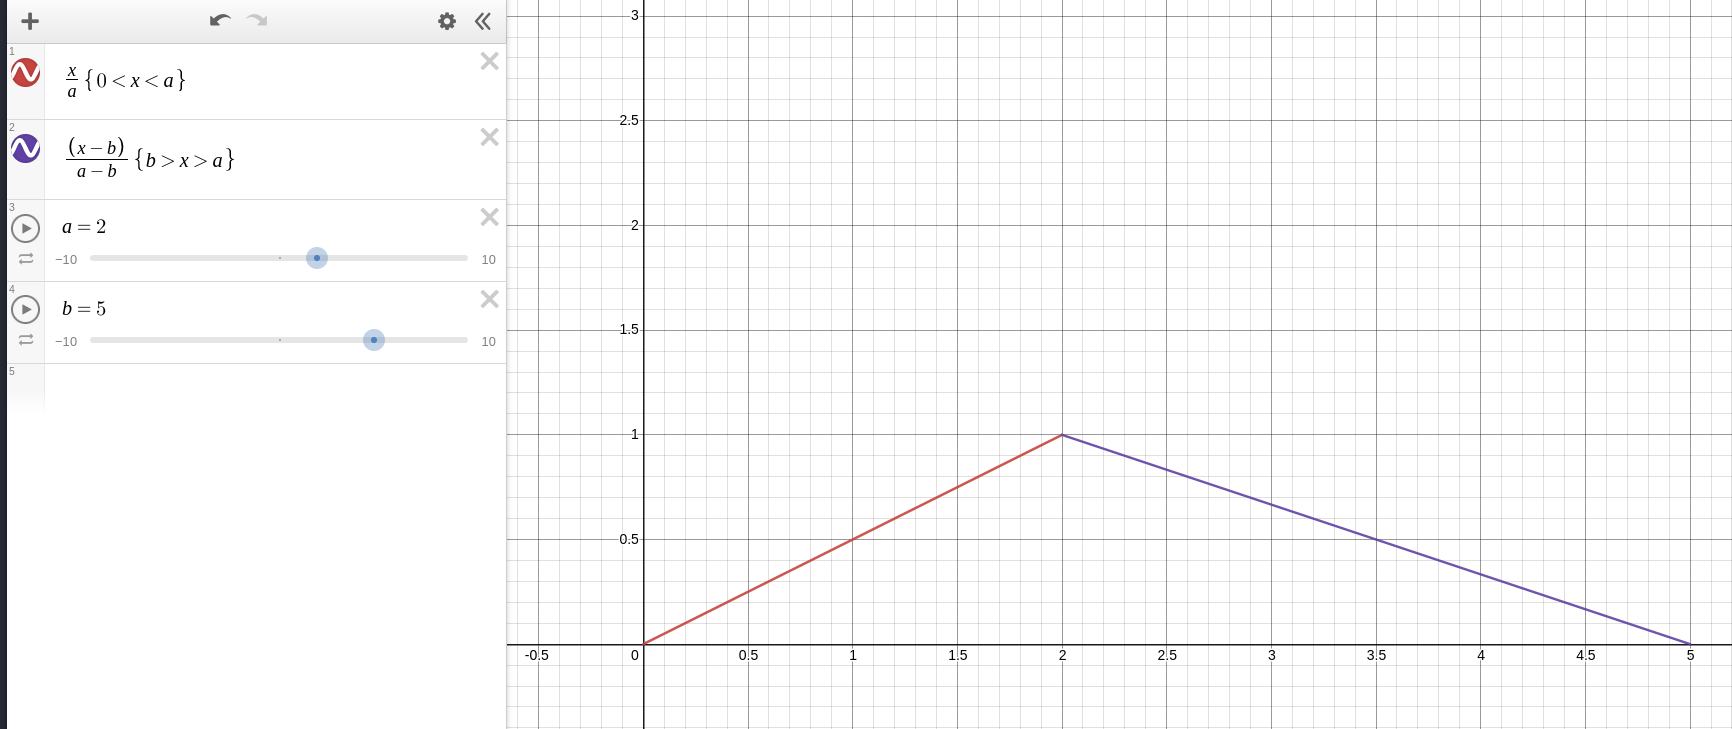
\includegraphics[width=0.8\textwidth]{q3}
    \caption{Graph of the wavefunction for question 3, here with $a=2$ and $b=5$}
    \label{fig:q3}
\end{figure}

{\noindent\bf Question 3c.} The expectation value is the tallest point of the wavefunction, so it is most likely to be found at $x=a$. 

{\noindent\bf Question 3d.} Compute the following integral: 

\[
\frac{3}{b}\int_0^a \left( \frac{x}{a} \right) ^2dx=\frac{a}{b}
.\] 

As expected if $a=b$ then the probability is just 1, and if $b=2a$ then the probability is $\frac{1}{2}$. 

{\noindent\bf Question 3e.} This is the same integral as part a except with an addition $x$ in front of it: 

\[
\frac{3}{b}\left(\int_0^a x\left(\frac{x}{a}\right)^2dx + \int_a^b x\left(\frac{(b-x)}{b-a}\right)^2dx\right)=\frac{3a^2}{4b}+\int_{a-b}^0\frac{3(x-b)x^2}{(b-a)^2b}dx
.\] 

\[
=\frac{3a^2}{4b}-\frac{3(b-a)^2}{4b}+(b-a)=\frac{6a-3b+4b-4a}{4}=\frac{2a+b}{4}
.\] 

{\noindent\bf Question 4.} One device, or at least a protocol that has been proposed that uses quantum mechanics is quantum cryptography, specifically quantum key distribution. The purpose of this scheme is to generate a key known privately to two parties such that it is impossible for others to know. To enable this, quantum key distribution takes advantage of the observer effect present for all quantum situations. If an eavesdropper were to intercept the message used to generate the key, then it would be automatically be evident that someone had done so since the wavefunction of the data being passed would have collapsed. Thus if one party gets the information used to make the privately shared key, they have absolute certainty that it has not been looked at yet.  


\end{document}
